	%!TEX root = ../../Main.tex
\graphicspath{{Chapters/Krav/}}
%-------------------------------------------------------------------------------


\section{Krav til dynamiken}
I dette afsnit beskrives kravene til hvilken funktionalitet systemet har. 


I samarbejde med vejleder er der opstillet en række krav.
\begin{itemize}
\item Systemet kan regulere en horisontal vinkel på op til ±30 grader tilbage til vandret i ”overdelen” ±1 grad
\item Overshoot max 5\%
\item Risetime 0.2 sekund 
\item Settlingtime 1 sekund 
\item Stadtionær fejl 10\%  

\end{itemize}



Herunder vil vi vise et blokdiagram, som viser en beksrivelse af systemets (fysiske) blokke, som beskriver opbygningen af systemet på Lego bilens styringsenhed. 


\begin{figure}[H]
	\centering
	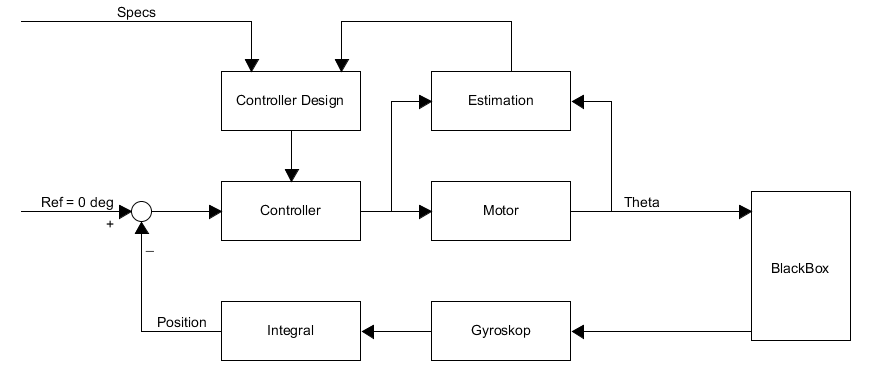
\includegraphics[width = 400 pt]{Img/blokdiagram.png}
	\caption{Blokdiagram}
	\label{fig:Blokdiagram}
\end{figure}
